%%%%%%%%%%%%%%%%%%%%%%%%%%%%%%%%%%%%%%%%%
% Short Sectioned Assignment
% LaTeX Template
% Version 1.0 (5/5/12)
%
% This template has been downloaded from:
% http://www.LaTeXTemplates.com
%
% Original author:
% Frits Wenneker (http://www.howtotex.com)
% License:
% CC BY-NC-SA 3.0 (http://creativecommons.org/licenses/by-nc-sa/3.0/)
%
%%%%%%%%%%%%%%%%%%%%%%%%%%%%%%%%%%%%%%%%%

%----------------------------------------------------------------------------------------
%	PACKAGES AND OTHER DOCUMENT CONFIGURATIONS
%----------------------------------------------------------------------------------------

\documentclass[paper=a4, fontsize=10pt, font=arial]{scrartcl} % A4 paper and 11pt font size
\usepackage[T1]{fontenc} % Use 8-bit encoding that has 256 glyphs
\usepackage{fourier} % Use the Adobe Utopia font for the document - comment this line to return to the LaTeX default
\usepackage[english]{babel} % English language/hyphenation
\usepackage{amsmath,amsfonts,amsthm} % Math packages
\usepackage{url}
\usepackage{sectsty} % Allows customizing section commands
\allsectionsfont{\centering \normalfont\scshape} % Make all sections centered, the default font and small caps
%\graphicspath{ {figures/} }
\usepackage{geometry}
\usepackage{float}
\usepackage{graphicx}
\usepackage{caption}
\usepackage{subcaption}
\usepackage{cite}
\usepackage{fancyhdr} % Custom headers and footers
%\usepackage{movie15}
%\bibliographystyle{unsrt}
\pagestyle{fancyplain} % Makes all pages in the document conform to the custom headers and footers
\fancyhead{} % No page header - if you want one, create it in the same way as the footers below
\footskip=0pt
\hoffset=0pt
\fancyfoot[L]{} % Empty left footer
\fancyfoot[C]{} % Empty center footer
\fancyfoot[R]{\thepage} % Page numbering for right footer
\renewcommand{\headrulewidth}{0pt} % Remove header underlines
\renewcommand{\footrulewidth}{0pt} % Remove footer underlines
\setlength{\headheight}{0pt} % Customize the height of the header
\setlength{\footheight}{0pt} % Customize the height of the header
\numberwithin{equation}{section} % Number equations within sections (i.e. 1.1, 1.2, 2.1, 2.2 instead of 1, 2, 3, 4)
\numberwithin{figure}{section} % Number figures within sections (i.e. 1.1, 1.2, 2.1, 2.2 instead of 1, 2, 3, 4)
\numberwithin{table}{section} % Number tables within sections (i.e. 1.1, 1.2, 2.1, 2.2 instead of 1, 2, 3, 4)
%\textheight=260cm
\setlength\parindent{11pt} % Removes all indentation from paragraphs - comment this line for an assignment with lots of text
\setlength{\parskip}{1em}
%----------------------------------------------------------------------------------------
%	TITLE SECTION
%----------------------------------------------------------------------------------------

\newcommand{\horrule}[1]{\rule{\linewidth}{#1}} % Create horizontal rule command with 1 argument of height

\title{	
\normalfont \normalsize 
\textsc{University of Derby, Department of Electronics, Mathematics \&\ Computing} \\ [25pt] % Your university, school and/or department name(s)
\begin{figure}[H]
\centering
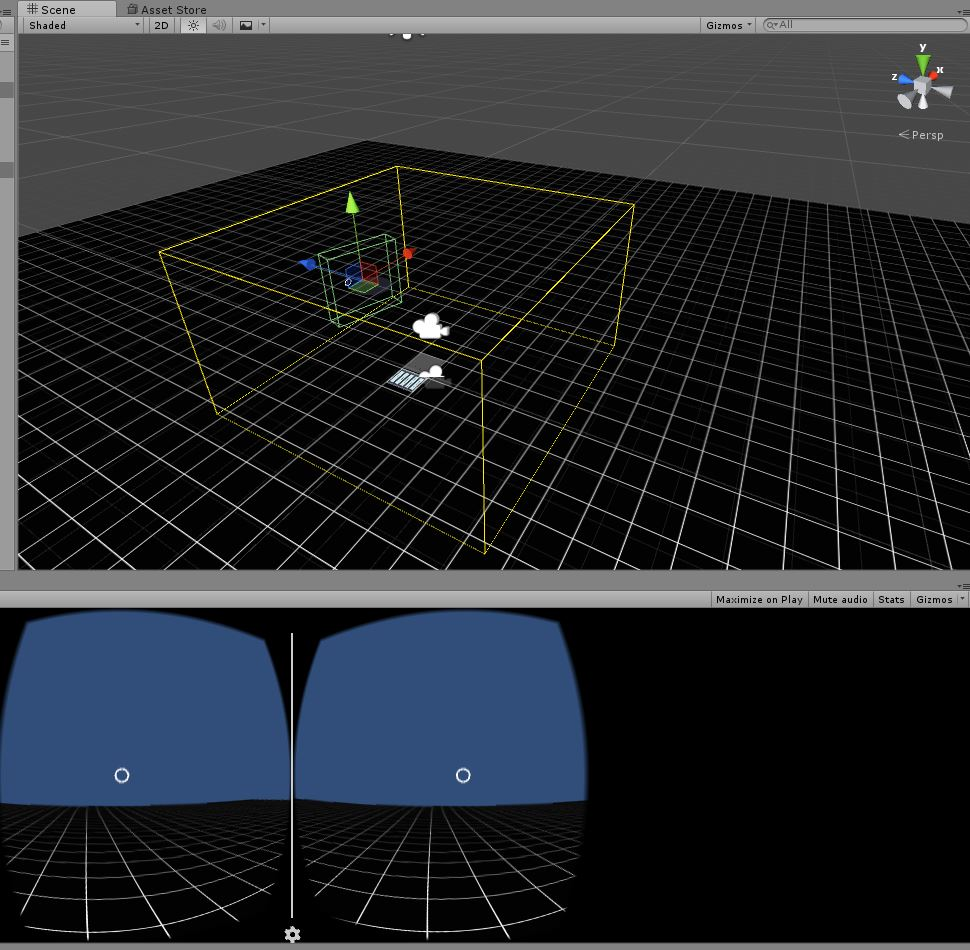
\includegraphics[width=0.5\textwidth]{overview_unity.jpg}
\centering
\caption{A screen-shot of the test interface design within unity, both in third person 'observer' and first person 'subject' views}
\end{figure}
\horrule{0.5pt} \\[0.4cm] % Thin top horizontal rule
\huge An Attempt to Implement a Listening Test to Quantify the Impact of Diffuse Reverberation Level on Localization in Modern VR Applications \\ % The assignment title
\horrule{2pt} \\[0.5cm] % Thick bottom horizontal rule
}

\author{Simon Durbridge} % Your name

\date{\normalsize\today} % Today's date or a custom date

\begin{document}

\maketitle % Print the title

\newpage

%----------------------------------------------------------------------------------------
%	Contents
%----------------------------------------------------------------------------------------

\tableofcontents

%\newpage

%----------------------------------------------------------------------------------------
%	Figures
%----------------------------------------------------------------------------------------

\listoffigures

\newpage

%----------------------------------------------------------------------------------------
%	Abstract
%----------------------------------------------------------------------------------------

%\section{Abstract}

%\newpage

%----------------------------------------------------------------------------------------
%	Introduction
%----------------------------------------------------------------------------------------

\section{Introduction}

Over the last few years a new wave of Virtual Reality(VR) technology has has become available, often utilising mobile devices as the playback medium. Along with development of the visual component of these VR systems, spatial audio techniques beyond stereo panning and similar abstractions are often being used to create immersive '3 dimensional' sound experiences.
In a previous report~\cite{Durbridge2016b}, faculties surrounding the localisation of sound sources within the auditory scene were described. It was suggested that early reflection were a key component used in sound source localisation, and literature suggested that appropriate simulation techniques would be required for accurate sound source localization in VR~\cite{Begault1995}. 


\subsection{Research Question}

Does the level of artificial diffuse reverberation have an impact on a listeners capacity to localise a sound source in a VR environment, with the use of a simple early reflection simulation method? When utilising a reverberation tool that combines direct reflection simulation and artificial diffuse reverberation, is it possible to counteract the effects of early reflections on localization accuracy by masking the direct reflections with an overly loud diffuse field?

Null Hypothesis: Diffuse reverberation level has no impact on sound source localization error in VR environments.

The aim of this study is to determine if a tool that combines direct reflection and diffuse reverberation simulation, is appropriate from a sound source localisation perspective in VR applications. In this study the Google virtual reality software development kit (VRSDK)~\cite{googlevr2016} for Unity was used for development of the listening test environment. The VRSDK version used was 1.0, and the version of unity used was 5.4.2f2.

\subsection{Report Overview}

Initially the experiment method will be discussed, and the behaviour of the GVRSDK room reverb algorithm will be explored. Following this, the experiment protocol will be given. Next, cursory experiment data will be analysed, and finally the experimental method will be reviewed and improvements suggested.


\newpage

%------------------------------------------------
\section{Experimental Method}

In order to analyse the tools available for new VR systems, it was considered crucial to develop a listening test that incorporated such a tool with as little modification to the tool as possible. Time constraints were also a factor in realising such a test, as little prior mobile application development experience was directly available. Given these constraints, the Unity game engine system was chosen as a development platform. This was beneficial as Unity has native Android and GVRSDK support~\footnote{Though due to instability, the most recent versions of Unity and GVRSDK were not used in the development of this experiment}.

The VR environment the test subject is placed in consists of a single ground plane, with an ancillary menu of simple functions such as Reset function, visual distortion correct and other functions relating to the visual system. The single ground plane appears to stretch out significantly far, to provide limited bias to room size. The reset function allows a user to skip to the next round of the test, if they cannot find the sound source. Test scores for the previous round of the test are also displayed on the plane, so that those administering the test can record the results without having to access the phone.

A $4*4*4meter$ cube sound source with a collider but no direct mesh is randomly moved to a position on a unit semi-sphere of random diameter, centred around the test subject who is held at the same point in space $1.5 meters$ above the centre of the plane. The sound source would have a relatively cardioid dispersion characteristic, and would always be oriented to face the test subject. An example of the sound source used can be seen in figure 2.1, with the cardioid pattern, green box collider and viewers reticle (cursor). The reticle is important in VR systems, as it allows users to always understand where their cursor is pointed. To compensate from the visual stimulus of the reticle allowing for easy accurate visual localization, the reticle is allowed to grow relatively small and the box collider is oversized. It was stressed to test subjects that the reticle is a visual guide that would not point directly at the centre of the sound source, and that localization should be based on the sound of the environment with an aim to find the centre of the sound source. Localization error is measured as the angle between the absolute centre of the sound source collider, and the direction in which the test subject is looking.

\begin{figure}[H]
\centering
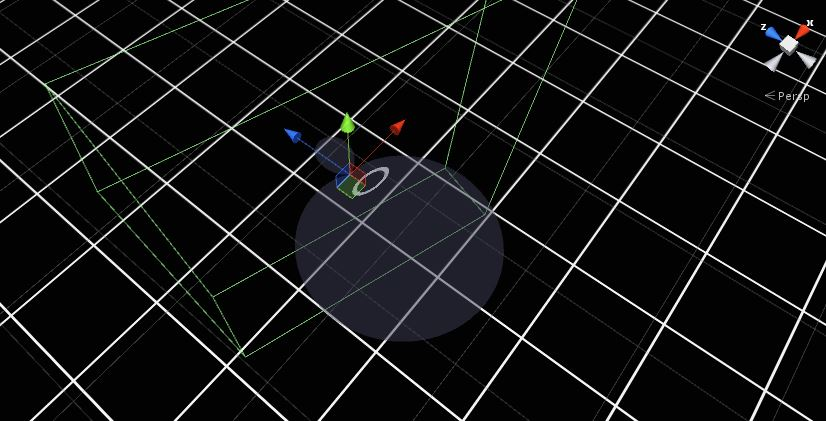
\includegraphics[width=0.7\textwidth]{dispersion-pattern.JPG}
\centering
\caption{A screen-shot of the sound source and its dispersion pattern}
\end{figure}

As the test progresses the size of the room in the reverberation model is increased, and the amplitude of the diffuse reverb component is varied.

	\subsection{Google VR SDK Reverb Engine}
Google have unsurprisingly minimal public documentation discussing how the proprietary GVRSDK GvrAudioRoom component models room reverb. There are however popular methods of calculating low-order direct (early) reflections using methods such as the image-source method, and [CITEME] suggested a reverb modelling method that uses a combination of the image-source method and all-pass reverberation to simulate room characteristics at low computational cost. The user is provided with 11 variable parameters for modelling room reverb:
\begin{itemize}
  \item Wall Material
  \item Reflectivity
  \item Gain
  \item Brightness
  \item Time
\end{itemize}
The first two parameters in the list appear to influence the intensity and length of the early reflection component, as can be seen in figure 2.2. The response shown are of the left receiver, and include the effects of the HRTF filtering used in the GVRSDK. The latter three parameters appear to effect the diffuse component of the reverberation. For the sake of this experiment, only the room size and diffuse reverb gain are altered. 

\begin{figure}[H]
\centering
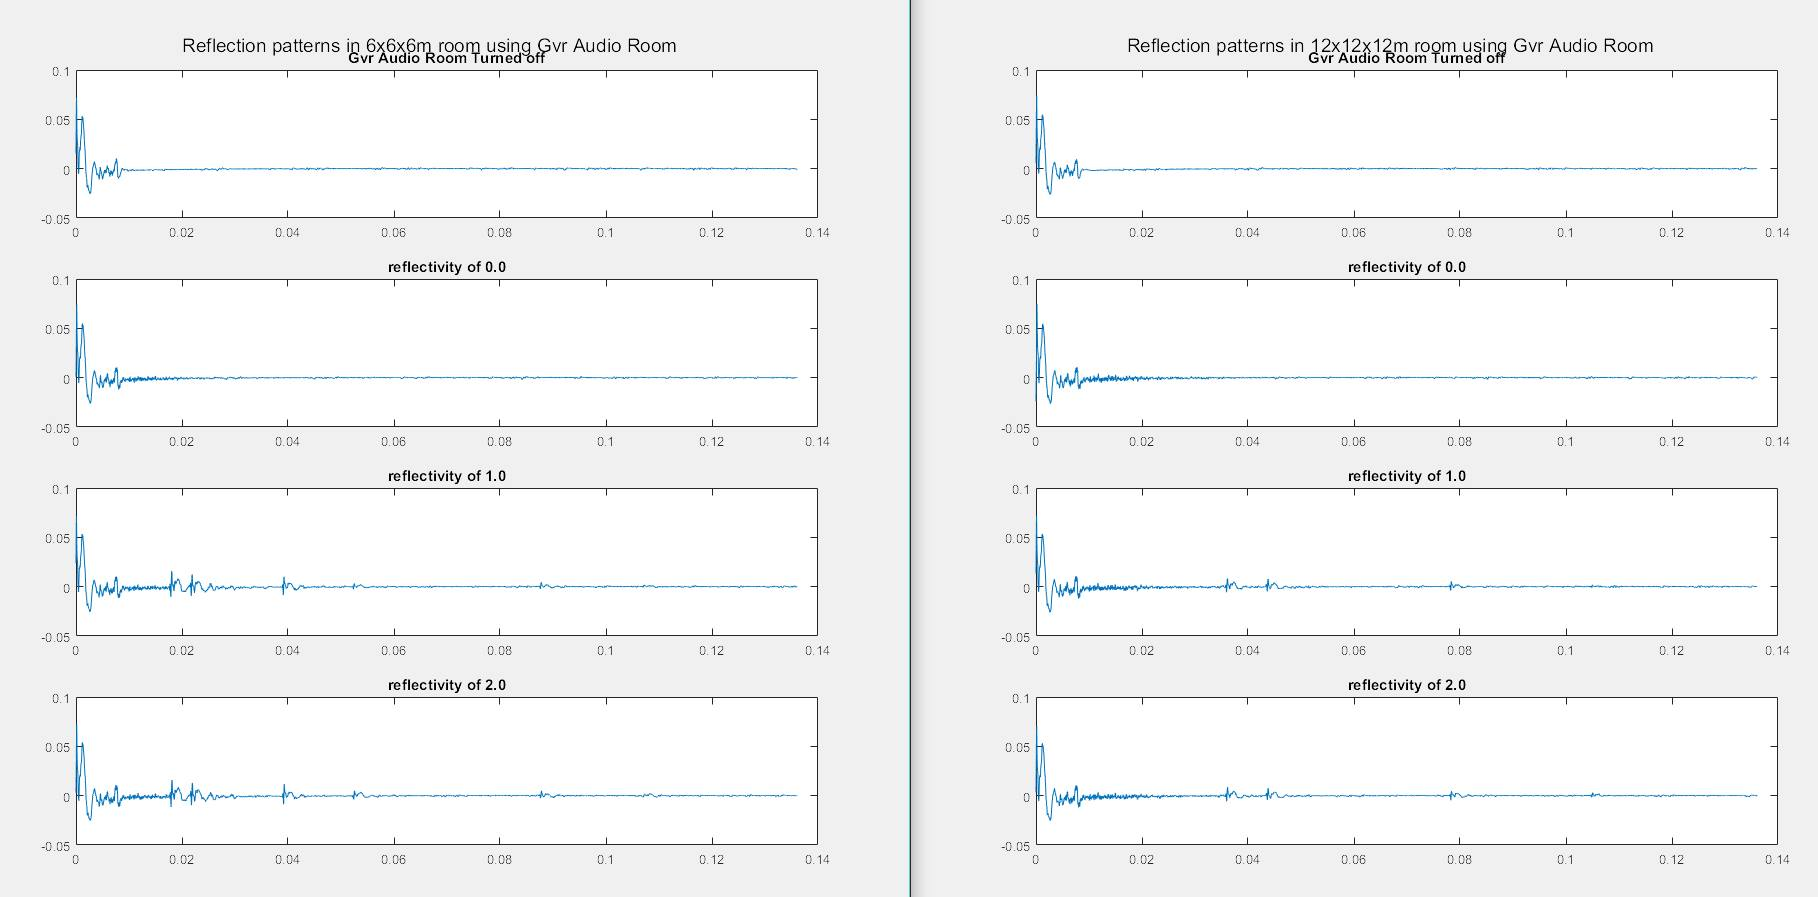
\includegraphics[width=1.0\textwidth]{ir6m12m.jpg}
\centering
\caption{Comparison plots of impulse response of 6m and 12m rooms with varying reflectivity and no diffuse reverberation}
\end{figure}


	\subsection{Experiment Protocol}
Test subjects were asked to evaluate three random source locations in each of three different surrounding room sizes. The room sizes were doubled each time, and the listener position was maintained at $1.5 meters$ above the ground plane. The audio sample used was a mono mix of an excerpt from a monologue by climber Chris Schulte, made for the JamCrack Podcast and used with permission of podcast owner Niall Grimes \footnote{ \url{http://www.niallgrimes.com/jam-crack-podcast/jcpc-006-the-view-from-dead-horse-point}}. This audio sample was used as the content was simple and clear, with a reasonable consistency of quiet periods to allow for the decay of the reverb to be heard. The audio room size began at $7 meters$ by $7 meters$ by $4 meters$, and increase to twice as large each time.

\section{Results and Evaluation}
	\subsection{Results}


	\subsection{Evaluation}


\section{Experiment Review}

One of the many issues with this test revolved around the need for the reticule as a cursor, thus having to compensate for the reticule by over-sizing the sound source object. The reticule was implemented due to a limited understanding of the triggering mechanics in Unity and the GVRSDK. The reticle must be triggered by hitting the box collider and having the user press the cardboard trigger, in order for the game engine to enter the method for moving the sound source and displaying the results. For an implementation with a relevantly large sample set, a different triggering mechanism should be implemented that is compatible with the 'on trigger' part of the GVRSDK set of functions but is not attached to the reticle directly. 

In relation to the reverberation modelling component of the GVRSDK, it would have been preferable to implement an algorithm that included a modifiable early reflection order. This would have allowed for a test of localization error due to reflection order as well as if those reflections could be masked with diffuse reverb.

Later versions of the GVRSDK have some added functionality for the GvrAudioSource and GvrAudioListener objects that are not available in the version used in this test. As these versions of the GVRSDK become more stable, it would be preferable to implement them in a later test. 

\section{Conclusion}


%----------------------------------------------------------------------------------------
\newpage
\section{References}

\bibliography{mybib}{}
\bibliographystyle{plain}

\end{document}